\subsection{Implementación del firmware de adquisición}

El firmware de adquisición constituye la primera capa ejecutable del sistema. Su papel es transformar la salida digital del ADS1299 en una señal EEG preparada para el backend Python. Para ello configura el convertidor, espera a que haya una nueva conversión disponible, lee el frame por SPI, reconstruye las muestras, las escala a unidades físicas, aplica un filtrado digital básico y agrupa los datos en bloques mediante el evento \texttt{eeg\_block\_uV}.

Dentro del flujo general del sistema, esta capa se encarga de las tareas más cercanas al hardware y al tiempo real. El microcontrolador asegura que las muestras lleguen a Python con una cadencia coherente, en microvoltios y con una estructura de bloque estable. A partir de esos bloques, el backend Python realiza el almacenamiento temporal, el análisis espectral, la evaluación de calidad y la generación de parámetros para la sonificación.

La Figura~\ref{fig:impl_firmware_flujo_adquisicion} resume esta cadena de transformación de datos, desde el frame nativo del ADS1299 hasta el bloque \texttt{eeg\_block\_uV} consumido por el backend Python.

\begin{figure}[H]
    \centering
    \IfFileExists{images/uml/impl_firmware_flujo_adquisicion.pdf}{%
        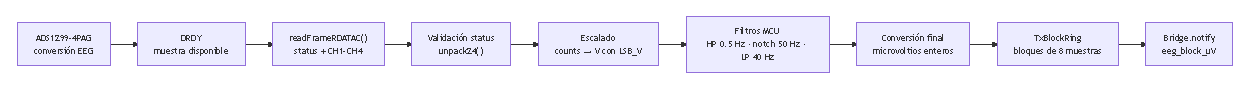
\includegraphics[width=0.92\textwidth]{images/uml/impl_firmware_flujo_adquisicion.pdf}
    }{%
        \fbox{\parbox{0.9\textwidth}{\centering Diagrama pendiente de exportar desde Mermaid: \texttt{images/uml/impl\_firmware\_flujo\_adquisicion.mmd}}}%
    }
    \caption{Flujo de adquisición implementado en el firmware. El microcontrolador lee frames RDATAC del ADS1299, valida el campo de estado, reconstruye las muestras de 24 bits, las escala, aplica filtrado digital y publica bloques de 8 muestras hacia Linux.}
    \label{fig:impl_firmware_flujo_adquisicion}
\end{figure}

La implementación se reparte en varios archivos. \texttt{sketch.ino} actúa como programa principal: inicializa Bridge, Monitor, ADS1299, filtros y handlers de comunicación, y ejecuta el bucle de adquisición. La clase \texttt{ADS1299\_SafeSPI} encapsula el transporte SPI de bajo nivel. El driver \texttt{ADS1299Plus} implementa la secuencia de arranque, los comandos, el acceso a registros y la lectura de frames. El archivo \texttt{ADS1299\_Registers.h} recoge comandos, direcciones y máscaras del ADS1299 con nombres legibles. Por último, \texttt{filters.h} contiene el acondicionamiento digital en el microcontrolador y \texttt{streaming.h} define la estructura de bloque, la cola de transmisión y la publicación hacia Linux.

\subsubsection{Configuración del ADS1299}

El ADS1299-4 es un convertidor analógico-digital de cuatro canales, 24 bits y muestreo simultáneo, orientado a señales EEG y biopotenciales. Internamente integra un amplificador de ganancia programable, una referencia de tensión, un oscilador y un filtro digital de decimación. La comunicación con el microcontrolador se realiza mediante una interfaz compatible con SPI, por lo que el firmware puede configurar registros y leer muestras mediante comandos digitales.

En este proyecto el ADS1299 trabaja a \SI{250}{\hertz}, con ganancia 24 y referencia interna de \SI{4.5}{\volt}. La ganancia 24 se utiliza porque las señales EEG son de muy baja amplitud y deben amplificarse antes de la conversión digital. La tasa de \SI{250}{\hertz} fija el ritmo común de adquisición: el convertidor produce una muestra nueva aproximadamente cada \SI{4}{\milli\second}. Aunque el dispositivo permite otras tasas de datos, en esta implementación se usa una única frecuencia global para todos los canales.

La configuración se realiza en dos niveles. Primero, \texttt{ADS1299Plus::begin()} deja el dispositivo en un estado conocido: configura pines, inicializa SPI, aplica \texttt{RESET}, detiene conversiones previas, entra en \texttt{SDATAC} y lee el registro de identificación. Esta lectura permite comprobar que el dispositivo pertenece a la familia ADS1299 y que la variante detectada es de cuatro canales, coherente con el contrato de adquisición usado por firmware y Python.

Después, \texttt{configureDefaults()} programa una configuración base mediante registros como \texttt{CONFIG1}, \texttt{CONFIG2}, \texttt{CONFIG3}, \texttt{CHnSET}, \texttt{BIAS\_SENSP}, \texttt{BIAS\_SENSN}, \texttt{LOFF\_SENSP} y \texttt{LOFF\_SENSN}. Estos nombres proceden del mapa de registros del ADS1299 y evitan que el código principal dependa de valores binarios opacos. Los comandos principales empleados por el driver son \texttt{RESET}, \texttt{START}, \texttt{STOP}, \texttt{RDATAC}, \texttt{SDATAC}, \texttt{RREG} y \texttt{WREG}. \texttt{RREG} y \texttt{WREG} se usan para leer y escribir registros; \texttt{SDATAC} detiene la lectura continua durante la configuración; y \texttt{RDATAC} activa el modo de lectura continua usado durante la adquisición.

En la versión final del prototipo se utiliza \texttt{ADS\_DIAGNOSTIC\_MODE=5}. Este modo mantiene CH1 como canal EEG principal, con entrada normal y ganancia 24. Los canales CH2--CH4 permanecen dentro del frame para conservar el contrato estructural de cuatro canales, pero se configuran apagados o cortocircuitados y no se interpretan como canales EEG activos finales. La derivación de BIAS se limita a CH1P y CH1N, y la detección \textit{lead-off} se desactiva durante la captura final para no inyectar señales diagnósticas en la señal usada para la sonificación.

\begin{table}[H]
    \centering
    \caption{Configuración final del ADS1299 en el modo de adquisición empleado.}
    \label{tab:impl_ads1299_modo_final}
    \begin{tabular}{p{0.22\textwidth}p{0.33\textwidth}p{0.34\textwidth}}
        \hline
        \textbf{Elemento} & \textbf{Configuración final} & \textbf{Papel en la adquisición} \\
        \hline
        CH1 & Activo, ganancia 24, entrada normal & Canal EEG principal usado por el procesamiento y la sonificación. \\
        CH2--CH4 & Apagados/cortocircuitados en el modo final & Conservados en el payload por contrato, sin interpretarse como EEG activo principal. \\
        BIAS & Derivado de CH1P + CH1N & Referencia de modo común limitada al canal usado. \\
        \textit{Lead-off} & Desactivado & Evita inyección diagnóstica durante la captura final. \\
        Test interno & Desactivado & No se mezcla señal de prueba con la señal real. \\
        Tasa de muestreo & \SI{250}{\hertz} & Frecuencia común entre firmware y backend Python. \\
        \hline
    \end{tabular}
\end{table}

Esta distinción evita una ambigüedad importante: el sistema mantiene un formato de datos de cuatro canales porque el ADS1299-4, el firmware, las capturas y el backend comparten ese contrato. Sin embargo, la validación experimental final se centra en CH1 como canal fisiológico principal.

\subsubsection{Sincronización temporal mediante DRDY y RDATAC}

Una vez configurado el ADS1299, el firmware inicia la adquisición manteniendo activa la señal \texttt{START} y enviando el comando \texttt{RDATAC}. En este modo, el convertidor genera frames de forma continua. La señal \texttt{DRDY}, activa a nivel bajo, indica que una nueva conversión está lista para ser leída.

El firmware no genera muestras por temporización software. Sigue el ritmo impuesto por el ADS1299. Cuando \texttt{DRDY} baja, una interrupción muy breve incrementa el contador \texttt{drdy\_count}. La lectura SPI no se realiza dentro de la interrupción, porque una ISR debe ser corta y no conviene ejecutar operaciones de comunicación, filtrado o publicación en ese contexto. Después, el bucle principal consulta el contador y, si existe una conversión pendiente, llama a \texttt{ADS1299Plus::readFrameRDATAC()}.

Cada frame RDATAC leído en esta configuración ocupa \SI{15}{\byte}: tres bytes de estado y cuatro canales de tres bytes cada uno. El driver baja \texttt{CS}, transfiere quince bytes por SPI enviando \texttt{0x00} como byte de relleno y vuelve a subir \texttt{CS}. El resultado se separa en un campo \texttt{status24} y cuatro muestras de canal.

La Figura~\ref{fig:impl_secuencia_drdy_rdatac} resume esta secuencia. La clave es que \texttt{DRDY} solo marca disponibilidad de dato; la transformación de la muestra se realiza después en el bucle principal.

\begin{figure}[H]
    \centering
    \IfFileExists{images/uml/impl_secuencia_drdy_rdatac.pdf}{%
        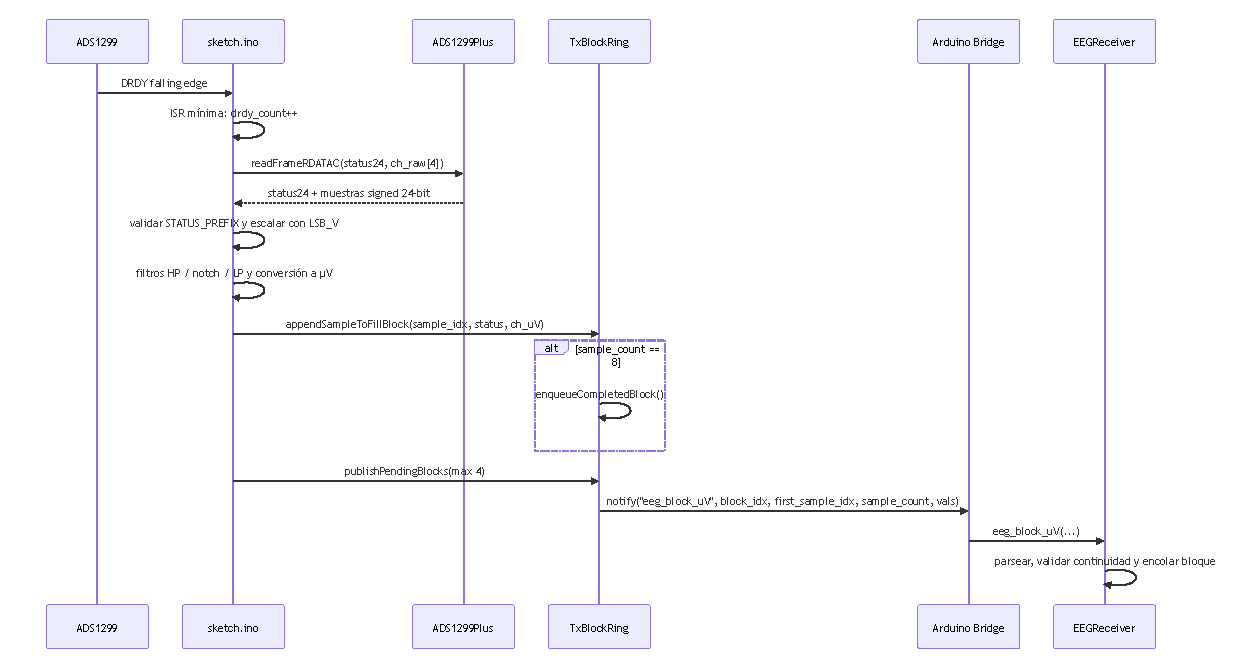
\includegraphics[width=0.98\textwidth]{images/uml/impl_secuencia_drdy_rdatac.pdf}
    }{%
        \fbox{\parbox{0.9\textwidth}{\centering Diagrama pendiente de exportar desde Mermaid: \texttt{images/uml/impl\_secuencia\_drdy\_rdatac.mmd}}}%
    }
    \caption{Secuencia simplificada de adquisición. La interrupción de \texttt{DRDY} solo marca la disponibilidad de una muestra; la lectura SPI, el filtrado y la publicación del bloque se realizan posteriormente en el bucle principal.}
    \label{fig:impl_secuencia_drdy_rdatac}
\end{figure}

\subsubsection{Reconstrucción, escalado y filtrado de muestras}

Cada frame RDATAC comienza con un campo de estado de 24 bits. El firmware valida que los bits más significativos coincidan con el prefijo esperado \texttt{0xC00000}. Esta comprobación permite detectar frames incoherentes o problemas de sincronía en la comunicación SPI antes de que la muestra avance por la cadena.

Después del estado aparecen las muestras de canal. Cada canal se transmite como tres bytes en orden \textit{MSB first}. El driver reconstruye esos tres bytes mediante \texttt{unpack24()} y realiza la extensión de signo a 32 bits. Este paso es necesario porque el ADS1299 entrega valores con signo: una muestra negativa debe seguir siendo negativa al almacenarse como \texttt{int32\_t}. Si no se extendiera correctamente el bit de signo, una muestra negativa podría interpretarse como un valor positivo de gran magnitud.

Una vez reconstruidas las cuentas digitales, el firmware aplica el factor \texttt{LSB\_V}. En la configuración utilizada, este factor vale \SI{2.235e-8}{\volt} por cuenta. Por tanto, la transformación física inicial es:

\[
    v = \text{cuentas ADC} \cdot \texttt{LSB\_V}
\]

La señal resultante todavía se mantiene en voltios dentro del microcontrolador para aplicar el acondicionamiento digital. La cadena de filtrado se aplica por canal y consta de tres etapas: un bloque de eliminación de continua o paso alto de \SI{0.5}{\hertz}, un filtro de muesca centrado en \SI{50}{\hertz} y un filtro paso bajo de \SI{40}{\hertz}. El primer filtro reduce la deriva lenta de línea base, el segundo atenúa la interferencia de red eléctrica y el tercero limita el contenido de alta frecuencia antes del análisis posterior.

Tras el filtrado, la muestra se convierte a microvoltios enteros mediante \texttt{volts\_to\_uV\_i32()}. Esta conversión deja la señal en una unidad natural para EEG y simplifica el contrato con Python: el backend ya no recibe cuentas crudas del ADC, sino valores físicos en microvoltios.

La Figura~\ref{fig:impl_frame_rdatac_a_bloque_uv} muestra la transformación entre el frame nativo del ADS1299 y el bloque que finalmente recibe Python. La figura ayuda a distinguir dos niveles: un frame RDATAC representa una muestra multicanal; un bloque \texttt{eeg\_block\_uV} agrupa ocho frames ya validados, escalados y filtrados.

\begin{figure}[H]
    \centering
    \IfFileExists{images/uml/impl_frame_rdatac_a_bloque_uv.pdf}{%
        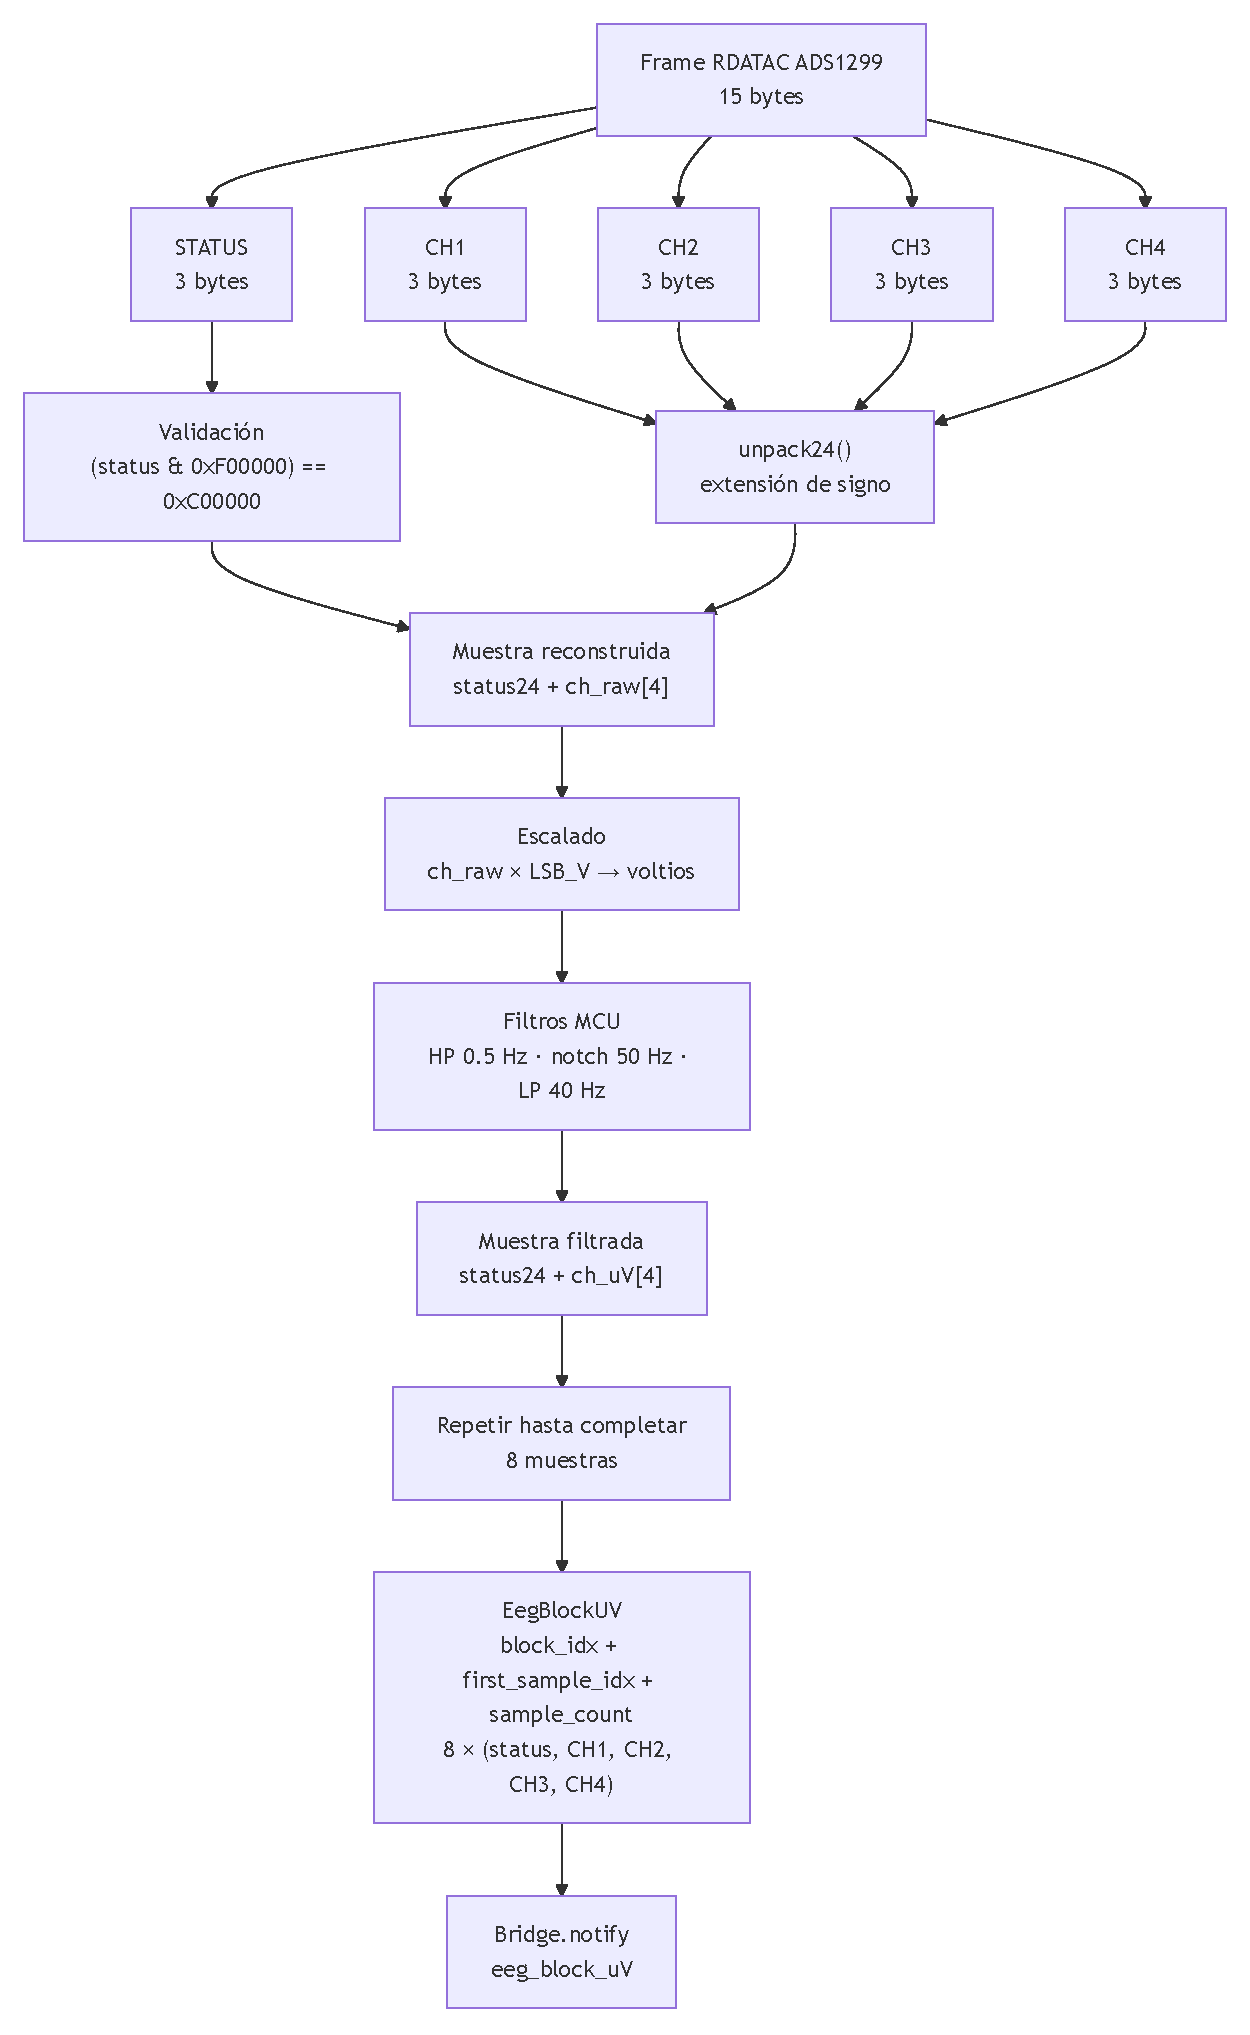
\includegraphics[width=0.90\textwidth]{images/uml/impl_frame_rdatac_a_bloque_uv.pdf}
    }{%
        \fbox{\parbox{0.9\textwidth}{\centering Diagrama pendiente de exportar desde Mermaid: \texttt{images/uml/impl\_frame\_rdatac\_a\_bloque\_uv.mmd}}}%
    }
    \caption{Transformación entre un frame RDATAC del ADS1299 y el bloque \texttt{eeg\_block\_uV}. Cada frame individual se valida, se reconstruye, se escala y se filtra; después se acumulan ocho muestras para formar el bloque enviado a Python.}
    \label{fig:impl_frame_rdatac_a_bloque_uv}
\end{figure}

\subsubsection{Agrupación y envío de bloques hacia Linux}

El firmware no publica una notificación por cada muestra individual. En su lugar, acumula ocho muestras filtradas en la estructura \texttt{EegBlockUV}, definida en \texttt{streaming.h}. Con una frecuencia de muestreo de \SI{250}{\hertz}, cada muestra representa \SI{4}{\milli\second} y cada bloque de ocho muestras representa \SI{32}{\milli\second}.

Cada bloque contiene una cabecera con \texttt{block\_idx}, \texttt{first\_sample\_idx} y \texttt{sample\_count}. Después incluye, para cada una de las ocho muestras, el \texttt{status} del ADS1299 y los cuatro canales expresados en microvoltios. Esta estructura es el contrato entre el firmware y Python.

\begin{table}[H]
    \centering
    \caption{Relación temporal entre muestra, bloque y transporte en la adquisición.}
    \label{tab:impl_tiempos_adquisicion}
    \begin{tabular}{p{0.28\textwidth}p{0.25\textwidth}p{0.36\textwidth}}
        \hline
        \textbf{Elemento} & \textbf{Valor} & \textbf{Significado} \\
        \hline
        Frecuencia de muestreo & \SI{250}{\hertz} & Una muestra nueva aproximadamente cada \SI{4}{\milli\second}. \\
        Tamaño de bloque & 8 muestras & Agrupación mínima antes de publicar por Bridge. \\
        Periodo nominal de bloque & \SI{32}{\milli\second} & Intervalo temporal representado por cada \texttt{eeg\_block\_uV}. \\
        Canales por muestra & 4 & Contrato estructural común a firmware, backend y capturas. \\
        \hline
    \end{tabular}
\end{table}

Cuando un bloque se completa, se introduce en una cola circular \texttt{TxBlockRing}. Esta cola desacopla la adquisición de la publicación por Bridge. Bridge es el mecanismo de comunicación entre el microcontrolador y el entorno Linux/Python de la UNO Q. Gracias a la cola, el firmware puede seguir adquiriendo muestras aunque el envío de un bloque concreto tarde algo más que una iteración del bucle.

La publicación se realiza mediante \texttt{Bridge.notify("eeg\_block\_uV", ...)}. En cada notificación se envía la cabecera del bloque y los datos de las ocho muestras. Además, el firmware limita el número de bloques publicados por iteración para evitar ráfagas excesivas hacia Linux.

La Figura~\ref{fig:impl_payload_eeg_block_uv} representa la estructura lógica del payload. Esta figura es especialmente importante porque cualquier cambio en este formato obligaría a modificar de forma coordinada el firmware, el receptor Python, las capturas CSV y las herramientas de validación.

\begin{figure}[H]
    \centering
    \IfFileExists{images/uml/impl_payload_eeg_block_uv.pdf}{%
        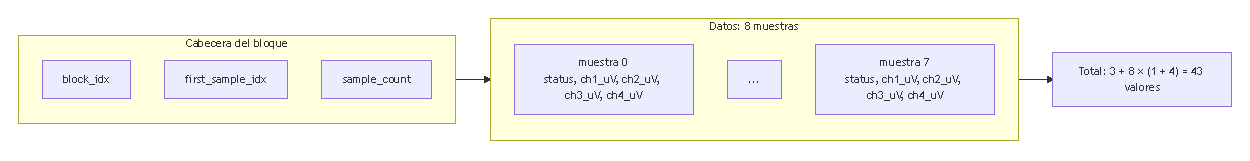
\includegraphics[width=0.86\textwidth]{images/uml/impl_payload_eeg_block_uv.pdf}
    }{%
        \fbox{\parbox{0.9\textwidth}{\centering Diagrama pendiente de exportar desde Mermaid: \texttt{images/uml/impl\_payload\_eeg\_block\_uv.mmd}}}%
    }
    \caption{Estructura lógica del evento \texttt{eeg\_block\_uV}. El firmware transmite una cabecera seguida de ocho muestras; cada muestra conserva el estado del ADS1299 y cuatro canales en microvoltios.}
    \label{fig:impl_payload_eeg_block_uv}
\end{figure}

En el lado Python, el contrato se centraliza en \texttt{eeg\_contract.py}. Este módulo define el nombre del evento, la frecuencia de muestreo, el número de canales, el tamaño de bloque, la máscara de estado del ADS1299 y el número esperado de campos. La función \texttt{parse\_eeg\_block\_values()} valida la longitud del payload y separa estados y muestras.

La clase \texttt{EEGReceiver}, implementada en \texttt{receiver.py}, registra el \textit{callback} \texttt{eeg\_block\_uV}. Este \textit{callback} se mantiene deliberadamente ligero: convierte argumentos a enteros, valida el payload, comprueba continuidad de índices, cuenta estados ADS1299 inválidos y encola el bloque completo. El procesamiento digital no se ejecuta dentro del \textit{callback}; el backend drena después la cola mediante \texttt{drain\_blocks\_to\_processor()} y entrega los bloques al procesador con \texttt{add\_block\_uV()}.

Con esta implementación, la frontera firmware--Python queda definida de forma precisa. El microcontrolador entrega bloques de ocho muestras, con cuatro canales en microvoltios y estado ADS1299 por muestra. Python valida y almacena esos bloques antes de transformarlos en ventanas de análisis. La siguiente parte del capítulo describe cómo el backend consume esta señal ya estructurada para calcular características espectrales y métricas de calidad.
